%%%% ijcai19-multiauthor.tex
\typeout{IJCAI-19 Multiple authors example}

% These are the instructions for authors for IJCAI-19.

\documentclass{article}
\pdfpagewidth=8.5in
\pdfpageheight=11in
% The file ijcai19.sty is NOT the same than previous years'
\usepackage{ijcai19}

% Use the postscript times font!
\usepackage{times}
\usepackage{soul}
\usepackage{url}
\usepackage[hidelinks]{hyperref}
\usepackage[utf8]{inputenc}
\usepackage[small]{caption}
\usepackage{amsmath}
\usepackage{booktabs}
\urlstyle{same}
%%
% FIGURES
\usepackage{graphicx}
\graphicspath{./figs}
\usepackage{grffile} % to set right names of files
%%
% CAPTIONS
\usepackage{caption}
\usepackage{subcaption} % supersedes subfigure & subfloat. try using options
%%
% LISTS
\usepackage{enumitem} %\begin{itemize}[leftmargin=*]
%% inline
\newlist{inline}{enumerate*}{1}
\setlist[inline]{before=\unskip{: }, itemjoin={{; }}, itemjoin*={{; and }}, label={(\roman*)}}
\usepackage{silence}
\WarningFilter{ctable}{Transparency disabled:}
\WarningFilter{xcolor}{Incompatible color}
\usepackage[usenames,dvipsnames]{color}
\newcommand{\aacomment}[1]{({\color{magenta}AA: #1})}
\newcommand{\tuta}{\emph{T.~absoluta}}
\usepackage{etoolbox}
\newtoggle{short}
%%\toggletrue{short}

% the following package is optional:
%\usepackage{latexsym} 

% Following comment is from ijcai97-submit.tex:
% The preparation of these files was supported by Schlumberger Palo Alto
% Research, AT\&T Bell Laboratories, and Morgan Kaufmann Publishers.
% Shirley Jowell, of Morgan Kaufmann Publishers, and Peter F.
% Patel-Schneider, of AT\&T Bell Laboratories collaborated on their
% preparation.

% These instructions can be modified and used in other conferences as long
% as credit to the authors and supporting agencies is retained, this notice
% is not changed, and further modification or reuse is not restricted.
% Neither Shirley Jowell nor Peter F. Patel-Schneider can be listed as
% contacts for providing assistance without their prior permission.

% To use for other conferences, change references to files and the
% conference appropriate and use other authors, contacts, publishers, and
% organizations.
% Also change the deadline and address for returning papers and the length and
% page charge instructions.
% Put where the files are available in the appropriate places.

\title{Interpreting Complex System Dynamics Under Data Scarcity: An
Application to Invasive Species Spread}

%% \author{
%% First Author$^1$\footnote{Contact Author}\and
%% Second Author$^2$\and
%% Third Author$^{2,3}$\And
%% Fourth Author$^4$\\
%% \affiliations
%% $^1$First Affiliation\\
%% $^2$Second Affiliation\\
%% $^3$Third Affiliation\\
%% $^4$Fourth Affiliation\\
%% \emails
%% \{first, second\}@example.com,
%% third@other.example.com,
%% fourth@example.com
%% }

\begin{document}

\maketitle

\begin{abstract}
Networked agent-based models are being increasingly used to study spread of
diseases and invasive species. However, data scarcity coupled with
complexity of the model can lead to multiple explanations for the observed
phenomenon; simulation outputs very different from one another can closely
match the ground truth. Delimiting configuration subspaces that lead to
such variability helps identify knowledge gaps, and therefore guide data
collection and policy making. We present a novel framework to analyze
complex simulation systems using machine learning tools. It is applied to
the study of an invasive pest of tomato crop, \emph{Tuta~absoluta} that has
spread globally in the last decade threatening food security and social
welfare. Simulated spread patterns are clustered to capture variability.
The resulting clusters are further analyzed using decision trees to
discover relationship model parameters and the clusters. This work touches two emerging
topics in a novel way: machine learning aided simulation systems, and
explainable AI.
\end{abstract}

\section{Introduction}
Network dynamical systems have been effectively used to study large
interacting biological and social systems~\cite{adiga2018graphical}. In
some fields such as computational epidemiology~\cite{eubank2004modelling},
online social networks~\cite{guille2013information} and
transportation~\cite{transims}, they occupy a place among mainstream
modeling approaches.  These models are explicit algorithmic descriptions of
composed local interactions. The resulting dynamics of such a validated
model yields a causal description of the underlying complex system. A
potential challenge however is the large number of parameters used to
describe the system, particularly under data scarcity and model
uncertainty.  We propose novel ways to analyze the in which machine
learning algorithms can be applied to address these problems to increase
the utility of such models.  Here, we focus on the problem of invasive
species spread, in particular, pests and pathogens of important
agricultural crops.  Increasingly, network diffusion based models are being
applied to study such
phenomena~\cite{carrasco2010unveiling,nopsa2015ecological}.

With rapid increase in global trade and travel, an unintended side-effect
is the increase in the introduction of pests and pathogens at a global
scale. Biological invasions cause unprecedented disruptions to native
ecosystems~\cite{crowl2008spread} and health~\cite{pyvsek2010invasive}, and
threaten global food security~\cite{pimentel2001economic}. In the United
States alone, the annual economic costs due to environmental damages and
losses are over \$120B~\cite{pimentel2005update}. Invasive species directly
or indirectly impede the achievement of multiple goals sustainable
development goals drafted by the United Nations: zero hunger, no poverty,
good health and well being, climate action, etc.
From a modeling perspective, identifying possible pathways and routes of
introduction, assisting monitoring and mitigation efforts, understanding
the biology and ecology of the pest, and impacts of establishment and are
some of the important objectives~\cite{venette2010,cunniffe2015thirteen}.

The spread of pests and pathogens is driven by various natural and
anthropogenic factors.  Self-mediated dispersal (by flight or vector
assisted, wind), trade of host crops~\cite{hulme2009trade} and human
mobility are few examples.  Establishment depends on ecological
suitability: climate, presence of hosts, predators, etc. Traditionally,
modeling efforts have focussed on the latter
aspect~\cite{sutherst2000climate}. However, in the recent years, integrated
modeling efforts analyze multiple pathways have been
developed~\cite{soliman2012framework,carrasco2010unveiling}.
The challenge with such holistic approaches is that the models tend to be
complex and require multi-disciplinary effort, but data required for
calibrating and validating them (or their components) is scarce. This is
particularly a problem in the case of emerging pests and pathogens. In many
countries, the necessary infrastructre for detecting possible attacks is
absent~\cite{early2016global}. Market-to-market trade of crops is not
always documented, and therefore, has to be inferred through models
(structural uncertainty). For many aspects, functional relationships are
not clear (for example, trade volume and rate of spread).  

Due to model complexity coupled with knowledge gaps, it is possible that a
large number of model configuration explain the real-world observations. In
particular, simulation outputs very different from one another can closely
match the ground truth. Identifying this variability and relating it to
model parameters can inform the modeler and domain experts of knowledge
gaps and future research directions to reduce this uncertainty. In this
paper, we present a novel approach to understand and quantify this
epistemic uncertainty. We develop a modular framework that utilizes machine
learning algorithms to systematically analyze the phase space of complex
network dynamical systems. We apply it to study the spread of a devastating
pest of tomato, \emph{Tuta~absoluta} or the South American leafminer, which
has spread globally in the last decade and caused severe crop loss and
negative societal impact~\cite{biondi2017}. This work contributes in a
unique way to an emerging body of literature on the interplay of
data-driven models and mechanistic
models~\cite{lamperti2018agent}. \aacomment{something
about explainable AI if it is relevant.}

\section{Methodological framework}\label{sec:methods}
\newcommand{\conSpace}{\mathcal{C}}
\newcommand{\selectedConSpace}{\mathcal{C}_s}
\newcommand{\simSpace}{\mathcal{S}}
\newcommand{\selectedSimSpace}{\mathcal{S}_s}
\newcommand{\loss}{L_g}

%% From a procedural point of view, applying a simulation system to study any
%% phenomenon is a two-phase process. First phase involves parameterization,
%% verification and uncertainty quantification. This is followed by
%% application of the system
We present a framework to quantify and explain model uncertainty in a
simulation-based system. Figure~\ref{fig:clusterOutline} provides a
schematic diagram of the framework.  There are three main modules in the
framework. The first module is that of parameterization (calibration and
validation), where the parameter space is explored to identify
configuration subspaces that explain the ground truth. In the second
module, the selected simulation outputs are analyzed for variability in
output. A natural way of achieving this is by clustering them based on a
suitable distance measure. In the last module, these clusters are analyzed
with respect to configurations of the member simulation outputs.  We will
delve deeper into each module describing the challenges and research
directions. First, we will setup the notation for the network-based
simulation system.

\paragraph{Graph dynamical system.} Here, we will focus on network-based
diffusion models or graph dynamical systems~\cite{adiga2018graphical}, but
in general, the methods developed can be applied ot other simulation
systems as well. A graph dynamical system has the following form.
Let~$G(V,E)$ be a network on~$n$ nodes (directed or undirected). Each node
is assigned a state from a finite domain~$K$. To each node~$i$ we assign a
\emph{local transition function}~$f_i$ that determines its state at
time~$t$. This function is local in the sense that it only depends on the
state of node~$i$ and those of the neighbors of~$i$ in~$G$. This function
can be deterministic or stochastic and time varying. Network epidemic
models (SEIR)~\cite{newman2002spread} is a popular example class of such
systems. Let~$\conSpace$ denote (the set of all possible model
configurations.  Each configuration determines the local function, how
simulation is initialized, etc. For each configuration~$C$, let~$S$ be the
simulation output. The form of the output depends on the nature of model,
problem being addressed and ground truth.  For example, in a stochastic
simulation with Boolean node states,~$S$ might be a vector, where each
component~$S_i$ corresponds to the empirical probability that node~$i$ is
in state~$1$.
%%
\begin{figure}[htb]
\centering
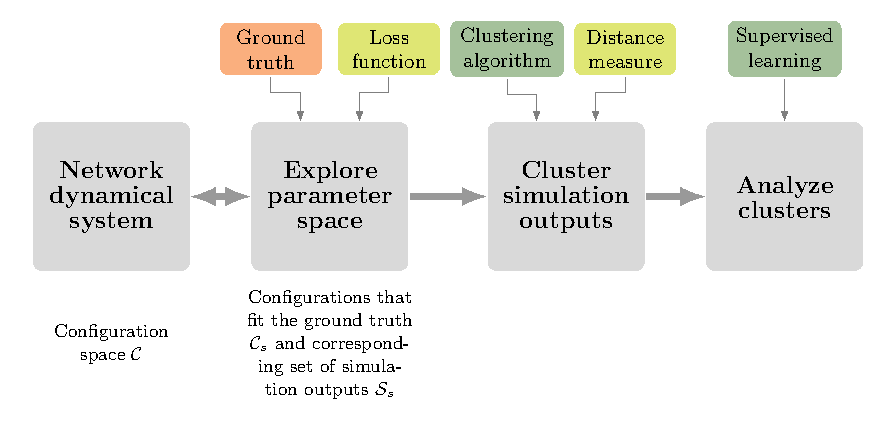
\includegraphics[width=1\columnwidth]{figs/spread_analysis.pdf}
\caption{Schematic of the simulation analysis framework. \label{fig:clusterOutline}}
\end{figure}
%%
\paragraph{Parameterization.} 
Calibration and validation of large-scale, high-resolution models is a
challenging task. Methods based on machine learning surrogates are being
increasingly used to accomplish this efficiently for complex agent-based
models~\cite{lamperti2018agent}. However, this aspect is outside the
scope of this work. Here, we will develop the necessary notation and
concepts required for the remaining part of the paper. This module explores
the parameter space~$\conSpace$ to identify configuration subspaces that
explain the ground truth. For a configuration~$C$, let the \emph{loss
function}~$\loss(C)$ denote a single-valued function that indicates
the goodness of fit of the configuration. It is evaluated by comparing the
simulation output with the ground truth. It could be a likelihood function
or a similarity score. We implicitly assume that the ground truth is at a
lower resolution compared to the simulation output. For example, it might
contain information about a strict subset of nodes or be aggregated
information such as number of nodes in a certain state. In addition,
uncertainty and inaccuracies in the dataset will have to be accounted for.
Given the configuration space~$\conSpace$, this module selects
configurations which explain the observations with regard to
$\loss(\cdot)$. The set of selected configurations is denoted
by~$\selectedConSpace$ and the set of corresponding simulation
outputs~$\selectedSimSpace$.
%%
\paragraph{Clustering simulation outputs.}
A natural way to analyze the variations in the selected configurations is
to cluster the simulation output. A similar approach was applied by
Cassandras~et~al.~(\citeyear{cassandras2000clustering}), albeit in a
different context. They use high-dimensional data clustering as an
interfacing component between simulation modules with different resolutions
in a multi-resolution simulation framework. Here, we cluster the space of
selected simulation outputs~$\selectedSimSpace$. Two important
considerations in this module are (i)~preprocessing simulation outputs and
(ii)~distance metric to compare two outputs. 

Let~$H(\cdot)$ denote the preprocessing function acting on simulation
outputs. Suppose~$S$ is a high-resolution output, this step potentially
includes simple operations such as normalizing its components in
preparation for clustering (preserving the resolution) to aggregation
operations (reducing the resolution). The form of $H(\cdot)$ is determined
by considerations such as nature of problem and computational issues. For
example, if the network has millions of components, directly
clustering~$\selectedSimSpace$ might be impractical.  We will assume that
$H(S)$ is at a higher resolution than ground truth.  For example, in the
context of infectious disease spread, ground truth can correspond to case
counts at the state-level and $S$ might be at the level of individuals.
Then, $H(S)$ can be case counts at the county level.

Given that the clustering represents uncertainty in the model, it is
critical to understand how choice of the clustering algorithm, number of
clusters and distance metric affect the outcome. In addition, parameter
exploration phase might influence cluster formation. Sampling too many or
too few configurationis from a configuration subspace can bias the
clustering.

\paragraph{Explaining model uncertainty.}

build notation;
clearly define the problem;
key challenges and research directions; possible that there are several
subspaces with the same simulation output.

\aacomment{an illustrative example?}

\paragraph{how this is related to explainable AI}

\section{Related work}
\paragraph{ABMs and ML in IAS.}
mainly ML has been used for ecological suitability
ABMs used for seed dispersal, human-mediated, seed networks ...
Garrett, Rebaudo, etc. to be just referred to
MAPSPAM
tuta specific models

Here we focus mainly on ABMs.

state of the art and emerging trends

\paragraph{Machine learning and Agent-based models.} In statistics,
surrogate modeling of complex simulation systems using Gaussian processes
is a well-studied area~\cite{linkletter2006variable}. Not only do the
surrogates replace the computationally intensive simulators, but they also
aid in analyzing the relative importance of variables. Recently,
Lamperti,~et~al.~(\citeyear{lamperti2018agent}) used a machine learning
surrogate (XGBoost). There are other ways in which researchers have
explored the integration of machine learning, scientific theories and
mechanistic models~\cite{van2017deep,karpatne2017theory}.

systems are
an emerging wawhere the . Compared to domains Network dynamical systems
we focus on invasive species spread, relatively new and emerging garrett,
13 challenges highlighting challenges

\paragraph{International trade networks.}


overfitting
high-resolution

only beginning to 
emerge~\cite{colunga2015following,tatem2009worldwide,ercsey2012complexity,
nopsa2015ecological,early2016global}.



spread. In the past decade, international and domestic trade and travel
send. In the past decade, international and domestic trade and travel
have been investigated [Ercsey-Ravasz et al., PloS One, 2012; Tatem et al.,
Proceedings of the Royal Society of London B: Biological Sciences, 2007].
There have been several attempts at holistic models to study particular
pests [Soliman et al., PloS One, 2012]. The field is also moving beyond
forecasting, with network- based models being applied to optimize
monitoring efforts [Nopsa et al., BioScience, 2015].
\section{An application to invasive species spread}
\newcommand{\pshort}{p_s}
\newcommand{\plocal}{p_{\ell}}
\newcommand{\pld}{p_{\ell d}}
\newcommand{\asd}{\alpha_s}
\newcommand{\afm}{\alpha_{\ell}}
\newcommand{\ald}{\alpha_{\ell d}}
\newcommand{\produce}{\mathrm{Prod}}
\newcommand{\veg}{\mathrm{V}}
\newcommand{\temp}{\mathrm{T}}
\newcommand{\consume}{\mathrm{Pop}}
\newcommand{\locality}{\mathrm{L}}
\newcommand{\export}{\mathrm{Export}}
\newcommand{\import}{\mathrm{Import}}
\newcommand{\process}{\mathrm{Proc}}
\newcommand{\moore}{\mathrm{M}}
\newcommand{\mooreRange}{r_\mathrm{M}}
\newcommand{\reportingCells}{\mathcal{C}_R}
\paragraph{Background}
\paragraph{Hierarchical model of spread.}
\paragraph{Parameterization and experiment design.}
Each model configuration was evaluated by comparing the simulation output
with \tuta{} incidence reports. We have incidence information from eight
locations in Bangladesh where pheromone traps were installed
(Figure~\ref{fig:bgdClassA}). The spread was simulated with infestation
starting from the location of first report (Panchagarh, Bangladesh). For
each cell, the empirical probability that it is in state~$I$ at time~$t$
was computed (averaged over 100 repetitions). The output was compared with
ground truth using a loss function adapted
from~\cite{carrasco2010unveiling}. Let~$v$ be a reporting cell and~$t_v$
denote the month of actual report of pest presence. To account for
uncertainty in reporting, we consider a time
window~$U_\tau=[t_v-\tau,t_v+\tau]$ during comparison, where~$\tau$ is the
uncertainty parameter. We set~$\tau=2$, i.e., error within $\pm2$ months is
tolerated. Supposing~$\reportingCells$ is the set of cells corresponding
to ground truth,  and ~$p(v,t)$ is the empirical probability that cell~$v$
is infected at time~$t$ in the model, then, the similarity~$\loss$ is given
by,
%%
\begin{align}\label{eqn:similarity}
    \loss(C)=\sum_{v\in\reportingCells} \Big(\sum_{t\in U_\tau}p(v,t)
    + \sum_{t\notin U_\tau}\big(1-p(v,t)\big) \Big)\,.
\end{align}
%%
The range or values of model parameters are in 
\iftoggle{short}{\cite{long}.}{Table~\ref{tab:param}.}
Parameter space exploration was conducted in multiple iterations.  First,
we coarsely sampled the space. With model parameters as independent
variables and loss function as as the dependent variable, we used
Classification and Regression Trees (CART) approach to identify subspaces
for which similarity score was high and rejected subspaces for which
similarity was low. Based on this, in the subsequent phases, we refined our
search to improve the parameterization. Simulations were performed on
more than~$500,000$ parameter combinations using a high performance
computing cluster.

\paragraph{Cluster analysis.}
2 clusters
more than 2 clusters
multi-type clusters
\paragraph{Sensitivity analysis.}
%%
\begin{figure}[t]
\centering
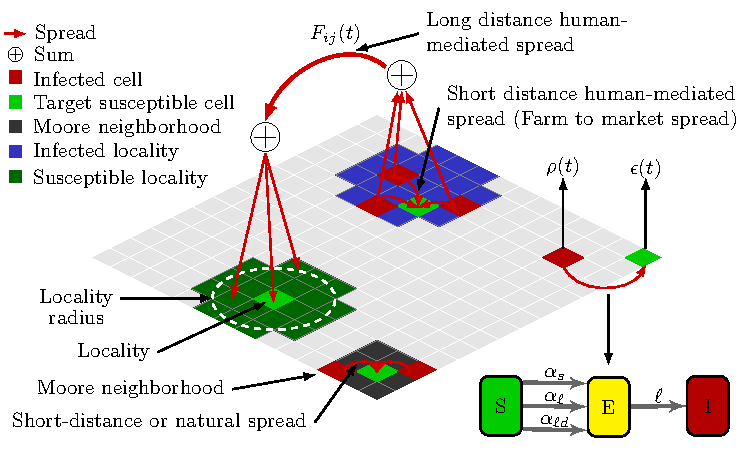
\includegraphics[width=\columnwidth]{figs/model_schematic.pdf}
\caption{\textbf{Multi-scale model of invasive species spread.} The
network structure, pathways and dynamics are captured in the illustration.
Also shown are the states and factors that influence state transitions:
infectiousness of a neighbor, suitability of the cell for pest
establishment, pathway parameters and latency period.
\label{fig:modelConcept}}
\end{figure}
%%
\begin{figure*}[!t]
\centering
\begin{subfigure}[b]{.32\textwidth}
    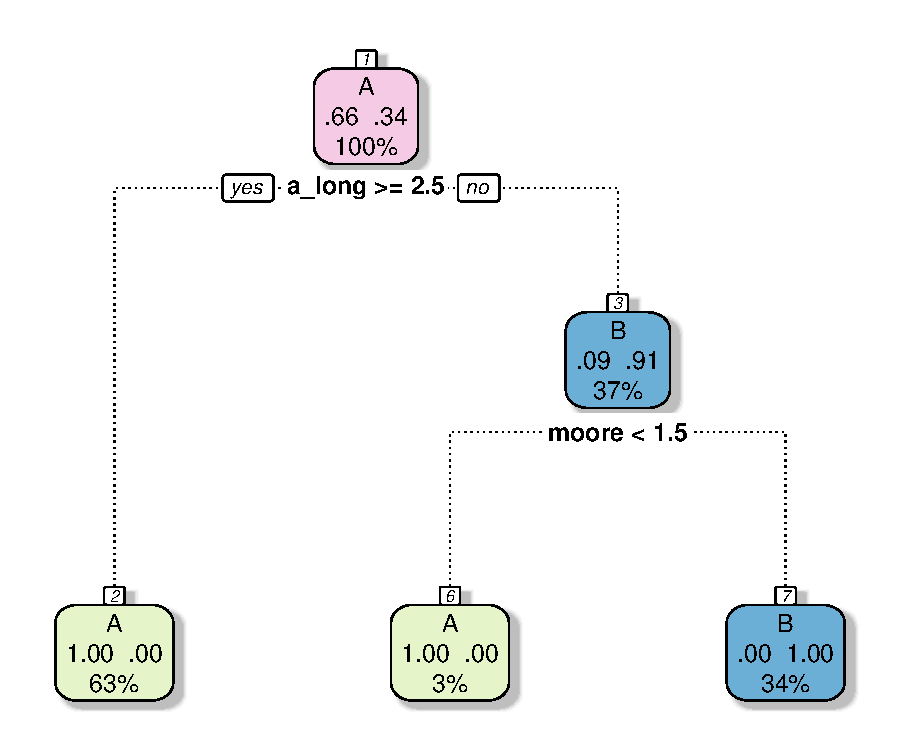
\includegraphics[width=\textwidth,trim=.6cm .6cm .6cm .6cm,clip]{../clustering/results/agglomerative/cart_cAB_agg.pdf}
\caption{$k=2$}
\end{subfigure}
\begin{subfigure}[b]{.32\textwidth}
    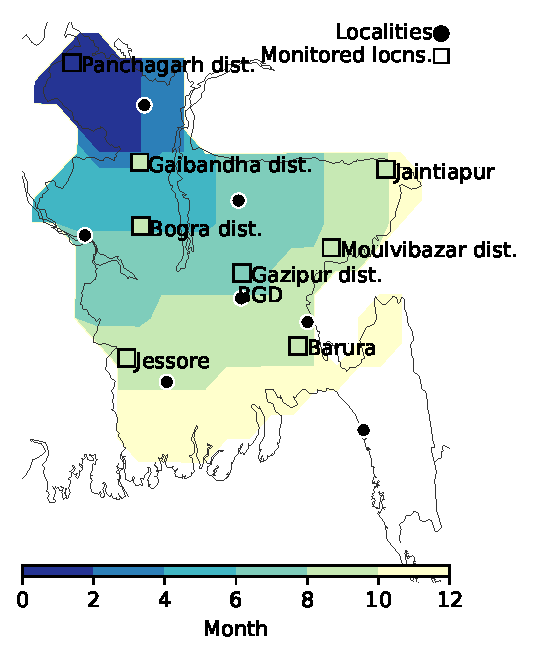
\includegraphics[width=\textwidth]{../cellular_automata/results/contour/BGD_model-A.pdf}
    \caption{Cluster~A \label{fig:bgdClassA}}
\end{subfigure}\hspace{.25cm}
\begin{subfigure}[b]{.32\textwidth}
    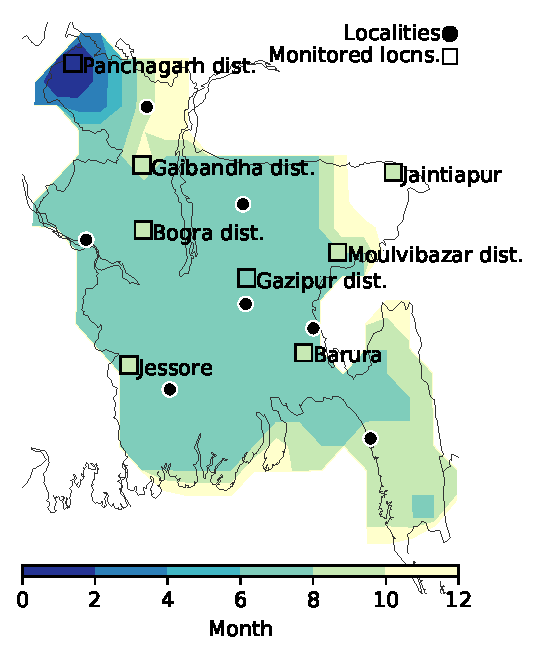
\includegraphics[width=\textwidth]{../cellular_automata/results/contour/BGD_model-B_m1_l3.pdf}
    \caption{Cluster~B \label{fig:bgdClassB1}}
\end{subfigure}
\caption{\textbf{Differenc.}The contour plots show the simulated
spread starting from the location of first report in Panchagarh district
for 12 months. For the purpose of plotting, the time of infection for a
cell is the minimum time step~$t$ such that the empirical probability that
the cell is infected by time~$t$ is $\ge0.8$. Also highlighted are the
eight monitored locations and the localities applied in the model. The
colors of the monitored locations correspond to the month of report
relative to the first report (Panchagarh). Two distinct spread patterns
emerged from the cluster analysis. (a) and (b) show representative spreads
observed for each class.}
\end{figure*}

%%
\section{Conclusion}

\clearpage
\bibliographystyle{named}
\bibliography{refs}
%%
\clearpage

\iftoggle{short}{}{
\appendix
%%
\begin{table}[t]
\caption{Model parameters and their values.\label{tab:param}}
    \centering
	\small
%% \rowcolors{2}{white}{gray!15} % For this to work, put \PassOptionsToPackage{table}{xcolor} before \documentclass
    \begin{tabular}{p{.093\textwidth}p{.33\textwidth}p{.5\textwidth}}
    %{cp{.25\textwidth}p{.25\textwidth}lr}
		\hline		
		Parameter & Description & Value/range \\
\hline		
\hline
$\mooreRange$ & Range of Moore neighborhood & $\{1,2,3\}$ corresponding to
spread per month of 
approximately~$25$kms,~$50$kms and~$75$kms
respectively. \\
%% $\suitable$ & Suitability threshold \\
$\ell$ & Latency period to transition from $E$ to $I$ & $\{1,2,3\}$ months
based on time for the pest to complete life cycle. \\
Monthly production & Disaggregation of annual production to monthly values
& \emph{Uniform} throughout the year or \emph{seasonal} based on regression
analysis (Methods). \\
$\beta$ & Gravity model distance function exponent & $\{0,1,2\}$ \\
$\kappa$ & Gravity model distance function cut-off & Between $4$ to $16$ hours
of travel time. \\
Seed & Location of initial infestation & \\
Locality radius & Determines cells assigned to a locality & 100kms \\\hline
$t_s$ & Time step of initial infestation & $\{3,4,5\}$ corresponding
to March, April and May respectively based on first report in
Bangladesh~\cite{hossain2016first}. \\
%% $\infest$ & Infectivity of a cell based on amount of production & \\
$\asd$ & Short-distance spread scaling factor & In the interval $[0,500]$.\\
$\afm$ & Local human-mediated dispersal scaling factor & In the interval $[0,500]$.\\
$\ald$ & Long distance spread scaling factor & In the interval $[0,500]$.\\
\hline
\end{tabular}
\end{table}
}
%%
\end{document}

